\chapter{Degeneration}
\label{cha:Degeneration}
Innerhalb dieses Kapitels wird der Ansatz der \textit{Degeneration} vorgestellt.

Die Benennung schöpft sich aus der Nähe zu genetischen Algorithmen \cite{heistermann2013genetische}, allerdings aus einer invertierten Perspektive: Um auf unbekannte Modelle einzugehen, wird hierbei von einem korrekt erkannten Bild \textit{weggearbeitet}. Anstatt allerdings \textit{gute Gene} zu kombinieren \cite{schoneburg1994genetische}, wird wird eine Genmutation erzeugt und überprüft, ob diese den Anforderungen der Klassifizierung noch genügt. 

Zunächst wird das Konzept anhand von Pseudocode genauer erläutert. Anschließend wird die Implementierung eines Algorithmus vorgestellt, der das unbekannte \ac{NN} des Wettbewerbs verwendet. Den Abschluss dieses Kapitels bildet eine lokale Implementierung inklusive einiger Verbesserungen, welche sich aufgrund der Limitierungen des Zugriffes auf die \textit{remote-AI} des Wettbewerbs nicht angeboten haben.
\section{Konzept}
\label{sec:DegenerationKonzept}
Die grundlegende Idee des Algorithmus bezieht sich darauf, ein Urbild $i$ zu einem Abbild $\hat{i}$ zu manipulieren, welches von dem unbekannten Klassifizierungsalgorithmus weiterhin korrekt erkannt wird. Abhängig von der Stärke der Manipulation soll eine $Tiefe$ gewählt werden, ab welcher der Algorithmus beendet wird. Als Beispiele der Manipulation seien insbesondere Rauschen und Glätten genannt, allerdings auch Kantenschärfung und Veränderungen der Helligkeit und anderer Metaparameter. Mit fortschreitender Tiefe wird nahezu jedes Bild für den Menschen unkenntlich. Zusätzlich sollten allerdings weitere Parameter als Abbruchkriterien aufgenommen werden, konkret eine Anzahl an Gesamt-Iterationen der Manipulationsfunktionen und eine Abbruchbedingung, beispielsweise wenn keine weiteren Fortschritte erreicht werden.

\newpage
\paragraph{Pseudocode} ~\newline 
Folgende Parameter erwartet die (generische) Implementierung des Degeneration-Algorithmus: 
\begin{itemize}
	\item Einen Eingabewert $i$
	\item Eine Manipulations-Funktion $a : i \rightarrow \hat{i}$
	\item Eine Klassifizierungsfunktion $p : i \rightarrow \mathrm{R}$
	\item Eine gewünschte Tiefe $d$ (empfohlen, nicht notwendig)
	\item Eine Iterationszahl $its$ (empfohlen, nicht notwendig)
	\item Ein Schwellwert $t$ , um wie viel \% die Vorhersage schlechter sein darf, als das vorhergegangene Bild 
\end{itemize}
Auf einige der Punkte wird in den Anmerkungen gesondert eingegangen. ~\newline
\IncMargin{1em}
\begin{algorithm}
	\SetKwInOut{Input}{input}
	\SetKwInOut{Output}{output}
	\Input{i,a,p,d,its,t}
	\Output{$\hat{i}$, score}
	\BlankLine
	$depth  \leftarrow 0$, $loop \leftarrow0$ \;
	$s \leftarrow p(i)$\;
	$ii \leftarrow i , is \leftarrow s$ \;
	\While{$depth<d ~ || ~ loop <its$}{
		$ai \leftarrow a(i)$ \;
		$as \leftarrow p(ai)$ \;
		\If{$as >= is-t$}{
			$is \leftarrow as$\;
			$ii \leftarrow ai$\;
			depth++\;
		}
		loop ++\;
	}
	return ii,is\;
	
	\caption{Degeneration}\label{algo_degen}
\end{algorithm}\DecMargin{1em}
\newpage
\paragraph{Anmerkungen}~\newline 
Die Manipulationsfunktionen müssen genau ein Bild der Größe (x,y) erhalten, genau ein Bild der Größe (x,y) wiedergeben und (für die generischen Implementierungen) keine weiteren Parameter erhalten. Zusätzlich sollte die Manipulationsfunktion zufällige Elemente erhalten. Sollte eine einfache, idempotente Glättungsfunktion den Schwellwert nicht erfüllen, so wird niemals eine größere Tiefe erreicht.

Tiefe, Schwellwert und Manipulationsfunktion müssen aufeinander abgestimmt werden. Es gibt einige Funktionen, welche eine starke Veränderung hervorrufen, und für welche eine geringe Tiefe bereits ausreicht. Auf der anderen Seite dieses Spektrums können Funktionen, welche lediglich minimale Änderungen vornehmen, schnell große Tiefen erreichen, ohne ein merklich verändertes Bild hervorgerufen zu haben. Diese Parameter auszubalancieren obliegt dem Nutzer. Bei der Auswahl der Parameter sollte zusätzlich berechnet werden, wie groß die letztendliche Konfidenz ist, falls die maximale Tiefe erreicht wird. 

Innerhalb der Implementierungen sollte zusätzlich eine \textit{verbose}-Funktion eingebaut werden. Hiermit kann zum einen ein ergebnisloser Versuch frühzeitig erkannt werden und zusätzlich, ob der Algorithmus sich verklemmt hat. Üblicherweise kann man erkennen, wenn die Manipulationsfunktion \textit{zu stark}, beziehungsweise der Schwellwert zu niedrig gewählt ist.

\section{Implementierung Remote}
\label{sec:DegenerationRemote}
Im Rahmen des Wettbewerbs wird mit einer Rest-API gearbeitet, welche in Abschnitt \ref{sec:EigenschaftenTrasi} analysiert wird und besondere Herausforderungen mit sich bringt: 

\begin{itemize}
	\item Anfragen können fehlschlagen
	\item zwischen Anfragen muss ein Timeout liegen
	\item Mehrere Nutzer, welche die API mit dem gleichen API Key beanspruchen, blockieren sich
\end{itemize}
~\newline
Zusätzlich wird der Grundalgorithmus um die \textit{Verbose}-Funktion und eine History erweitert. Mithilfe der \textit{History} können nach der Ausführung des Algorithmus hilfreiche Plots erstellt werden. Diese ist in dem nachfolgenden Code in Listing \ref{lst:remoteDeg} nicht enthalten.
 
Ebenso ist anzumerken, dass ignoriert wird, welche Klasse zuerst erzeugt wird. Solange irgendeine Klasse mit einer passenden Konfidenz gefunden wird, gilt das Ergebnis als hinreichend. Im Normalfall bleibt es allerdings bei derselben Klasse. 

Die Klassifizierungsfunktion wird innerhalb der Remote-Degeneration durch einige Hilfsfunktionen umgesetzt. Diese bereiten ein als \textit{Bytearray} vorliegendes Bild auf und senden es an das Trasi-Webinterface. Dies geschieht in der Methode \textit{Scorer.Send\_ppm\_image(img)}. In der Antwort des Trasi-Webinterfaces befindet sich ein JSON-Array mit den Scores einiger Klassen des bewerteten Bildes. 

Die Hilfsmethode \textit{Scorer.get\_best\_score(response)} gibt den höchsten gefunden Score wieder.
\newpage
\begin{scriptsize}
\pythonexternal[caption=Quellcode der Remote Degeneration, label=lst:remoteDeg]{CodeSnippets/remoteDegenerationSnippet.py}
\end{scriptsize}
\newpage
\section{Ergebnisse Remote}
\label{sec:DegenerationErgebnisse}
In diesem Abschnitt werden die mit der Degeneration erzielten Ergebnisse in Bezug auf die Trasi-Schnittstelle vorgestellt. Zunächst werden einige positive Beispiele (Erfolge) gezeigt, anschließend wir auf einige Probleme, die aufgetreten sind, eingegangen und zuletzt wird ein kurzes Zwischenfazit gezogen. 
\paragraph{Positive Ergebnisse} ~\newline Die zuverlässigsten Ergebnisse werden mit einfachem Rauschen erzeugt. Die Abbildung \ref{fig:stoptiefe600} zeigt, dass zunächst vorallem die Pixel außerhalb des eigentlichen Schildes verändert werden. Dieses Verhalten wird erwartet. Die farbstarken bunten Pixel sind hierbei entstanden, da Werte welche die gültige Reichweite [0,255] verlassen, wieder zyklisch zurück in den Farbbereich geholt werden. Sollte ein Farbwert durch das Rauschen einen Wert -2 erreichen, wird er auf 253 gesetzt.  

\begin{figure}[h]
	\centering
	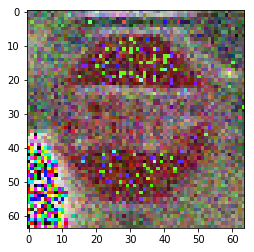
\includegraphics[width=0.4\linewidth]{Images/DegenSamples/StopTiefe600}
	\caption[Degeneration Tiefe 600]{Rausch - Degeneration mit 600 Iterationen}
	\label{fig:stoptiefe600}
\end{figure}

Während die Abbildung \ref{fig:stoptiefe600} noch als Verkehrsschild zu erkennen ist, führt ein längeres Ausführen der Degeneration zu einem Ergebnis wie in Abbildung \ref{fig:stoptiefe4000}. Um dieses Ergebnis zu erzielen wurden 4400 Sekunden benötigt, also ca. 73 Minuten.

\begin{figure}[h]
	\centering
	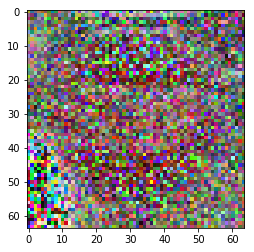
\includegraphics[width=0.4\linewidth]{Images/DegenSamples/StopTiefe4000}
	\caption[Degeneration Tiefe 4000]{Rausch - Degeneration mit 4000 Iterationen}
	\label{fig:stoptiefe4000}
\end{figure}

Die Plots in Abbildung \ref{fig:plotTiefe4000} stellen den Verlauf des Algorithmus dar: Das erste Diagramm zeigt einen Verlauf der aktuellen \textit{Tiefe} über die Iterationen, der zweite die jeweils produzierte Genauigkeit der jeweiligen Iteration (nicht nur die der akzeptierten), und der letzte Plot visualisiert diejenigen Iterationen, an welchen eine Änderung stattgefunden hat (weißer Strich) oder keine (schwarzer Strich). Innerhalb der Implementierung werden ebenfalls standardmäßig diese Plots erzeugt.

\begin{figure}[h]
	\centering
	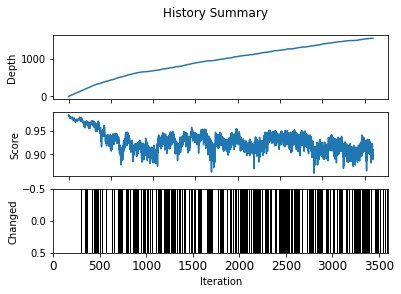
\includegraphics[width=0.6\linewidth]{Images/DegenSamples/StopTiefe4000Plot}
	\caption[Plot Degeneration]{Plot der Rausch-Degeneration}
	\label{fig:plotTiefe4000}
\end{figure}
Es wurden ebenfalls einige sehr positive Ergebnisse mit einer Mischung aus starkem Rauschen und Glätten erzeugt. Allerdings waren diese nicht zuverlässig reproduzierbar. 

\paragraph{Negative Ergebnisse} ~\newline Es gibt zwei primäre Fehlerquellen in Bezug auf die Remote-Degeneration: Die Auswahl von Bildern, welche im GTSRB-\textit{Training}-Set waren, sowie die Auswahl ungeeigneter Manipulationsfunktionen. 
~\newline
Das \ac{NN} des Wettbewerbs scheint sich die Bilder aus dem Trainingsset \textit{gemerkt} zu haben. Bereits minimale, unwichtige Änderungen des Schildes (z.B. Einfügen einiger blauer Punkte im Hintergrund) führen zu einer drastischen Verschlechterung des Ergebnisses. Dieses starke \textit{Ausschlagen} des Scores macht die Benutzung der Degeneration unbrauchbar.
\begin{figure}[h]
	\centering
	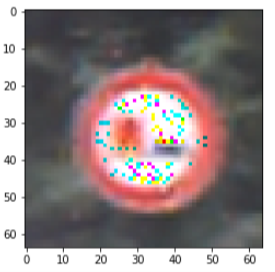
\includegraphics[width=0.5\linewidth]{Images/DegenSamples/OverFitSmaller}
	\caption[Degeneration overfit]{Rausch-Degeneration auf Trainingsbild - 36000 Iterationen}
	\label{fig:DegenOverfit}
\end{figure}
~\newline
Dieses Problem hat sich herauskristallisiert, als über einen längeren Zeitraum (\textasciitilde  10 Stunden) kein Bild erzeugt wurde, welches auch nur leicht verändert wurde. Die einzigen Änderungen, welche erzielt werden, befinden sich innerhalb des weißen Bereiches des Überholverbotsschildes, wie in Abbildung \ref{fig:DegenOverfit}. Es werden aber keine Änderungen außerhalb des Schildes vorgenommen, wo diese zu erwarten wären und bei vorhergehenden Versuchen auch zu beobachten sind (vgl. Abbildung \ref{fig:stoptiefe600}). 
~\newline
Dieses Problem tritt ausschließlich, allerdings zuverlässig, bei der Verwendung von Bildern aus dem Trainingsset auf. Es tritt nicht auf, sobald man Bilder aus dem Test-Set oder \textit{GTSRB-fremde} Bilder verwendet. Voraussetzung dabei ist, dass sie eine akzeptable Startkonfidenz besitzen. 

Innerhalb der lokalen Implementierung ist dieses Problem ebenfalls aufgetreten, konnte allerdings behoben werden, sobald man das Overfitting erkannt hatte.
\paragraph{Fazit} ~\newline
Innerhalb dieses kurzen Zwischenfazits sollen noch einmal die Vor- und Nachteile der Degeneration zusammengefasst werden:
\begin{table}[h]
	\centering
\begin{tabular}{|p{7.5cm}|p{7.5cm}|}
	\hline 
	\textbf{Vorteile} & \textbf{Nachteile} \\ 
	\hline 
	\textbf{Model-Agnostic:} \newline Der Algorithmus funktioniert unabhängig und ohne Wissen über das zugrundeliegende Modell & \textbf{Zeitintensiv:} \newline v.A. die Remote-Variante benötigt größere Zeitspannen \\ 
	\hline 
	\textbf{Kontext-Unabhängig:} \newline Die Herangehensweise ist nicht auf Bilderkennungen limitiert & \textbf{Vorwissen benötigt:} \newline Das Anwendungsfeld des zugrundeliegenden Models muss bekannt sein und ein geeignetes Startbild muss ausgewählt werden  \\ 
	\hline 
	\textbf{Erweiterbar:} \newline Die Manipulationsfunktionen können weiter ausgebaut werden und haben noch großes Potenzial & Die Degeneration erzielt bei empfindlichen Modellen schlechtere Ergebnisse - gerade sorgfältig trainierte Modelle sollten lange brauchen, um so überlistet zu werden \\ 
	\hline 
	\textbf{Simpel:} \newline Der Algorithmus ist einfach implementiert und erläutert, er benötigt keine höhere Mathematik oder Vorwissen zur Thematik \textit{Machine Learning} und der Modelle/Verfahren im Speziellen & Im Remote-Umfeld kann die Degeneration als DDoS wahrgenommen werden und entsprechend frühzeitig unterbunden werden. \\ 
	\hline 
\end{tabular} 
\caption{Zwischenfazit Degeneration}
\label{tab:FazitDegeneration}
\end{table}

Als besonderen Fall sind solche Modelle zu nennen, die mit jeder Anfrage \textit{hinzulernen}: ~\newline Diese sind entweder besonders anfällig gegenüber der Degeneration, weil sie die bereits veränderten Bilder als \textit{korrekt} klassifizieren und somit den Entstehungsprozess der Degeneration verinnerlichen oder sie \textit{härten} sich mit jedem Versuch gegen die neuen Änderungen und sind de facto immun gegen diesen Angriff.  

Solche permanent trainierenden Modelle sind in der Praxis allerdings selten im Einsatz, da sie für eine Vielzahl verschiedener Angriffe anfällig sind. Als einfaches Beispiel ist der Chatbot \textit{Tay} von Microsoft zu nennen: Dieser sollte angenehme Unterhaltungen mit Twitternutzern führen und aus den enstandenen Konversationen kontinuierlich weiterentwickelt werden \cite{mstay}. Innerhalb weniger Stunden gelang es einigen böswilligen Nutzern, dass Tay rassistische Äußerungen von sich gab \cite{mstaydown}. Microsoft hat den Service von Tay am zweiten Tag eingestellt. 
\section[Implementierung Lokal]{Implementierung Lokal \newline Anpassungen und Verbesserungen}
\label{sec:DegenerationLokal}

Innerhalb dieses Abschnittes werden zunächst die Änderungen bei der lokalen Verwendung des Algorithmus kurz behandelt und anschließend zwei konzeptionelle Verbesserungen vorgestellt: Parallel- und Batch-Varianten des Algorithmus. 

\paragraph{Anpassungen} ~\newline Für die lokale Implementierung wird zunächst von Grund auf ein eigenes Modell mithilfe der \ac{GTSRB}-Daten trainiert (siehe dazu Abschnitt \ref{sec:ImplAphrodite}). Das \textit{Scoring} der Remote-Implementierung wird durch die \textit{predict()}-Funktion des Models ersetzt.

Als zusätzliche Erweiterung wird für die lokale Implementierung umgesetzt, dass sich der Nutzer für eine bestimmte Klasse entscheiden kann, auf welche die Degeneration ausgelegt ist. Es wird also zuverlässig bspw. ein Stoppschild erzeugt und kein beliebiges Schild mit hohem Score. 

Des Weiteren entfällt die Wartezeit, welche zwischen Anfragen an die Schnittstelle benötigt wird. Auf diese Weise erhöht sich die Geschwindigkeit des Algorithmus maßgeblich. 

Eine zusätzliche, passive Verbesserung wird erzielt, indem die GPU-Acceleration Funktionen von Tensorflow verwendet werden. Diese beschleunigen nicht nur das Training des lokalen Models maßgeblich, sondern auch die Vorhersagen. Insbesondere die Batch-Variante konnte im Zusammenhang mit der eingesetzten NVIDIA Grafikkarte GTX 1070\footnote{https://www.nvidia.com/en-gb/geforce/products/10series/geforce-gtx-1070/} um den Faktor 20 beschleunigt werden.


\paragraph{Fazit}~\newline Das wichtigste Fazit, welches im Umgang mit der lokalen Implementierung gezogen werden kann, ist die Nichtverwendbarkeit der lokalen Bilder für die Schnittstelle. Während dies ursprünglich die Motivation war, schnell lokal Bilder zur Täuschung der "`Black Box"' des \ac{GI}-Wettbewerbs zu erzeugen und remote zu verwenden, stellte sich heraus, dass die lokalen Bilder keine guten Scores an der Schnittstelle erzielten und vice versa. 

Es ist anzunehmen, dass die Modelle dieselben Stärken haben bei der korrekten Erkennung von Verkehrsschildern, allerdings unterschiedliche \textit{Schwächen}. Die erzeugten Bilder zur Täuschung scheinen im Model selbst zu fußen und sind somit hochgradig spezifisch. 

Die meisten stark veränderten Bilder, welche i.A. nicht mehr vom Menschen als Verkehrsschilder erkannt werden, erzeugen bei dem \ac{NN}, welches im Algorithmus verwendet wird, Werte >90\%, und beim anderen Modell zuverlässig einen Score von $\approx$30\%. Für ein Bild, welches an sich nichts mehr mit einem Verkehrsschild zu tun hat, sind dies immer noch hohe Werte und die Zuverlässigkeit mit der dieser Zusammenhang auftritt lässt einen leichten, inhaltlichen Zusammenhang der Bilder erahnen.

\newpage
\subsection{Batch-Degeneration}
Innerhalb des Batch-Variante wird anstatt eines einzelnen Bildes ein Array aus $n$ veränderten Bildern erzeugt. 

Diese werden alle bewertet und falls das beste Bild des Batches den Schwellwert erfüllt wird mit dem besten Bild weiter gearbeitet. Dieses Verfahren entspricht deutlich näher der Genoptimierung von genetischen Algorithmen \cite{gerdes2013evolutionare}: Es wird aus $n$-Genen das beste ausgewählt. 

\begin{figure}[h]
	\centering
	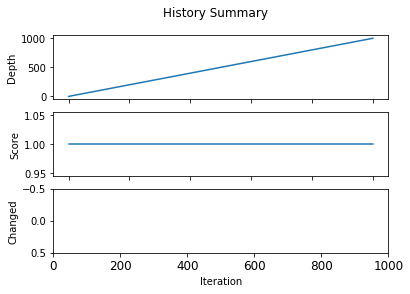
\includegraphics[width=0.5\linewidth]{Images/DegenSamples/BatchDegPlotTiefe1000}
	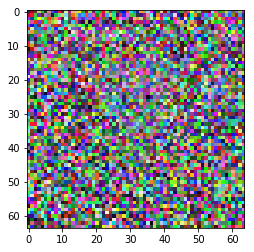
\includegraphics[width=0.35\linewidth]{Images/DegenSamples/BatchDegTiefe1000}
	\caption[Batch-Degeneration-Plot]{Verlauf der Batch-Degeneration mit Batchsize=10 und Tiefe=1000}
	\label{fig:batchdegplottiefe1000}
\end{figure}

Abbildung \ref{fig:batchdegplottiefe1000} zeigt den deutlich besseren Verlauf der Batch-Degeneration gegenüber der unveränderten Implementierung in Abbildung \ref{fig:plotTiefe4000}. Auffallend ist die durchgängige Veränderung und die gleichbleibend hohe Konfidenz von mehr als 99.9\% \footnote{Innerhalb des Plots wird es auf 1 gerundet}. Dieses Verhalten für die Webschnittstelle des \ac{GI}-Wettbewerbs einzusetzen ist möglich, allerdings wird aufgrund der Wartezeit zwischen den Anfragen davon abgesehen. 

Diese Variante profitiert maßgeblich von der \textit{GPU-Acceleration} innerhalb Tensorflows. Selbst ohne Verwendung des CUDA-Frameworks ist ein Tensorflow-Model auf Batch-Verarbeitung ausgelegt. Die optimale Batchgröße zu finden ist systemabhängig und sollte kurz getestet werden. Insgesamt benötigt die Batch-Degeneration trotzdem maßgeblich mehr Zeit: Für das Beispiel in Abbildung \ref{fig:batchdegplottiefe1000} werden ca. 15 Minuten benötigt, was knapp 5 mal so lange ist wie die ursprüngliche Implementierung. 

\textbf{Anmerkung:} Ein prinzipielles Problem der Batch-Degeneration liegt in der Zufälligkeit der Manipulationsfunktion. Als Beispiel sei einfaches Rauschen gewählt. Ein naheliegendes Verhalten für den Algorithmus ist von den 100 erzeugten Bildern dieses auszuwählen, welches das geringste Rauschen aufweist und als solches am wenigsten verändert wurde. Im Normalfall weist das am wenigsten veränderte Bild den nächsten Score auf. 

Glücklicherweise ist dies ein hypothetisches Problem und tritt in der tatsächlichen Implementierung nicht auf. Dennoch sollte es vor allem für die Manipulationsfunktion berücksichtigt werden. Im Falle einer Manipulationsfunktion, welche konstante Elemente beinhaltet (zum Beispiel Glätten oder statische Veränderungen der Helligkeit) fördert die Batch-Degeneration den selektiven Ansatz.
\subsection{Parallel-Degeneration}
Die Parallel-Variante stützt sich auf die Idee, mehrere Threads zu starten, welche gleichzeitig eine Degeneration durchführen.

Sobald ein einzelner Thread die gewünschte Tiefe erreicht hat, wird der Prozess beendet. 

~\newline Die Implementierung der Parallel-Degeneration ist aufgrund mehrerer technischer Gründe gescheitert: 

\begin{itemize}
	\item Modelgröße: Jeder Thread braucht ein eigenes Model, welches allerdings zu groß war. Naive Benutzung eines gemeinsamen Models führen zu Race-Con"-ditions, \textit{geschickte} Benutzung des Models führen zu einem Verhalten wie innerhalb der Batch-Variante
	\item Numpy-Arrays: Die Bilder für die lokale Degeneration lagen als Numpy-Arrays vor, welche ein besonderes Verhalten und eine besondere Benutzung innerhalb der Parallelverarbeitung benötigen \footnote{Dieses Problem ist sicherlich lösbar, allerdings ein Problem aus dem Bereich der Parallelverarbeitung, was im Kontext dieser Arbeit nicht weiter verfolgt wird.}. 
	\item Grafikkarteneinbindung: Sobald die GPU-Acceleration innerhalb Tensorflows eingerichtet ist, werden (nahezu alle) Anfragen an die Grafikkarte weitergeleitet. Diese unterstützt das parallele Verhalten der einzelnen Threads nicht. 
\end{itemize} 

Die Probleme sind hardware- oder frameworkbezogen. Je nach Umfeld können diese somit entfallen. Race-Conditions entfallen beispielsweise, wenn man in der Cloud arbeitet.

Diese Variante war für die Remote-Implementierung nicht umsetzbar, da gleichzeitige Anfragen (mit dem selben API-Key) fehlschlagen. Ein internes Scheduling der Anfragen führt nicht zu schnelleren Ergebnissen. 
\subsection{Tree-Degeneration}
Diese Variante führt eine Merkstruktur ein, welche die bisherigen Ergebnisse und Schritte zwischenspeichert. 

Das bisherige Verhalten entspricht dem einer Liste, bei welcher lediglich der letzte Knoten verwendet wird. Mit dem jeweils letzten Bild wird weitergearbeitet, bis entweder ein neues korrektes Bild erzeugt wird oder der Algorithmus endet. 
\begin{figure}[h]
	\centering
	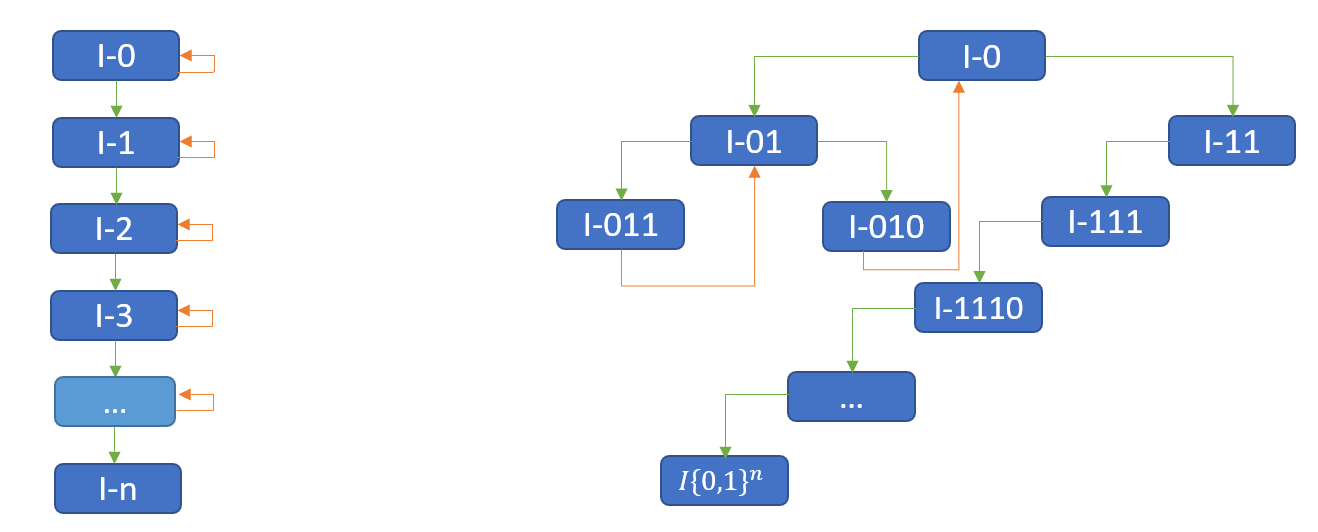
\includegraphics[width=0.8\linewidth]{Images/DegenTreeNormal}
	\caption[Tree-Degeneration]{Derzeitige Implementierung und eine baum-basierte Im"-ple"-men"-tie"-rung}
	\label{fig:degentreenormal}
\end{figure}

Die Variation beinhaltet das Führen eines \textit{Retry-Counters}, welcher bei jedem Versuch von einem Knoten erhöht wird. Sollte eine gewisse Anzahl an Versuchen ergebnislos bleiben, wird der aktuelle Knoten verworfen und der Vorgänger benutzt. 

Dieses Verhalten führt, je nach gewählter Maximalanzahl der Kinder eines Knotens, zu einem (Binär-)Baum. Das Abbruchkriterium der Tiefe kann weiterhin beibehalten werden und entspricht der Tiefe des Baumes. Im Falle eines versuchs- oder zeitbedingten Abbruchs wird das Bild mit der bisher größten Tiefe ausgegeben.

Die Entwicklung dieser Variante entstand durch die Beobachtung, dass die Geschwindigkeit der Degeneration stark abhängig sind vom Ausgangsbild. Es kann ein Bild erreicht werden, welches sehr \textit{sensibel} wahrgenommen wird und deutlich schwerer Änderungen \textit{toleriert}.

Die Batch-Degeneration ist mit dieser Variante frei kombinierbar.  